\chapter{5 Things Elon Musk Could Change About Twitter}

These notes follow a School of Hard Knocks interview, curated by LazyingArt LLC, and treat the lecture as a sequence of design conjectures about a platform rather than as settled platform history. There is no validated blackboard mathematics for this chapter, so when we write equations we are not transcribing a board; we are making explicit the accounting and incentive structure already carried by the speaker's argument. The lecture unfolds in a clear order: first motive, then bots, then authentication, then speech rules, then creator pay, then algorithmic openness, and finally the edit button as a problem of historical integrity.

\section{Why the Acquisition Matters}

The lecture begins not with a technical mechanism but with a divided audience. Musk's purchase of Twitter is presented as a split decision: some users are excited, others are anxious about where the platform may be taken. The speaker does not linger there. The disagreement is used to open a sharper question. If a figure this visible buys a platform that he already uses heavily, and if some of his tweets have already moved markets, then the purchase almost certainly carries purpose.

That is the first important shift in the lecture. We begin with public reaction, but we are quickly moved to strategic intention. The speaker points out that Musk runs major companies, participates in a number of other ventures, and sustains a celebrity brand of his own. From that he draws the natural inference that any such acquisition must come with responsibility, drive, and some notion of improvement. The frame widens for a moment to Musk's broader mission-oriented ventures, then narrows again. The lecture resets itself and promises a five-part breakdown of likely changes.

That reset matters. We are no longer asking merely what the public thinks. We are asking what sort of redesign an owner might attempt. In that sense, the chapter is about platform entrepreneurship: what gets measured, what gets cleaned up, what gets rewarded, and what must be preserved if the system is to remain credible.

\section{Bots, Metric Inflation, and the Case for Going Private}

\paragraph{From symptom to mechanism.}
The first predicted change starts exactly where many users would start: in the replies. We are asked to think of suspicious accounts, low-activity histories, recently created profiles, spammy comments, and scammy behavior. The lecturer begins with this local symptom because it is instantly recognizable. But he does not stay with anecdote for long. The pivot is immediate: bots are not just unpleasant. They distort the numbers by which the platform appears to succeed.

\begin{definition}
We let \(E_{\mathrm{rep}}\) denote reported engagement and \(M_{\mathrm{rep}}\) denote reported monthly active users. The lecture's bookkeeping logic is then captured by the decompositions
\begin{align}
E_{\mathrm{rep}} &= E_{\mathrm{auth}} + E_{\mathrm{bot}}, \\
M_{\mathrm{rep}} &= M_{\mathrm{auth}} + M_{\mathrm{bot}},
\end{align}
where the subscripts \(\mathrm{auth}\) and \(\mathrm{bot}\) distinguish authentic activity from bot-generated activity.
\end{definition}

This is a cautious reconstruction, but it matches the logic of the talk closely. If bots can like, retweet, comment, and post, then their actions enter the platform's headline metrics. In that sense the lecture is not merely about moderation. It is about contaminated accounting:
\begin{equation}
\text{Bot activity} \uparrow
\quad \Longrightarrow \quad
E_{\mathrm{rep}} \uparrow,\qquad
M_{\mathrm{rep}} \uparrow.
\end{equation}
The next step follows naturally. Reported engagement and reported user counts matter to shareholders. If those figures rise, the company can look healthier than it is. The lecture's claim is therefore sharper than ``bots are bad.'' It is that bots can help sustain a flattering report.

\paragraph{A worked accounting example.}
Suppose, just for illustration, that in a given period we have
\[
E_{\mathrm{auth}} = 120,\qquad E_{\mathrm{bot}} = 30,
\]
and
\[
M_{\mathrm{auth}} = 90,\qquad M_{\mathrm{bot}} = 10.
\]
Then the platform reports
\begin{equation}
E_{\mathrm{rep}} = 120 + 30 = 150,
\qquad
M_{\mathrm{rep}} = 90 + 10 = 100.
\end{equation}
If one later removes the bots, the underlying platform has not mysteriously collapsed. What has happened is that the gap
\begin{equation}
\Delta E = E_{\mathrm{rep}} - E_{\mathrm{auth}} = E_{\mathrm{bot}},
\qquad
\Delta M = M_{\mathrm{rep}} - M_{\mathrm{auth}} = M_{\mathrm{bot}}
\end{equation}
has been made visible rather than hidden.

This is the point at which the lecture brings in public ownership. One reason, the speaker says, to take Twitter private is that a public company must care about shareholder opinion and about how the company looks on paper. If bot activity helps elevate the visible counts, then private ownership creates room to clean the platform rather than defend the contaminated totals.

\begin{figure}[h]
\centering
\resizebox{\linewidth}{!}{%
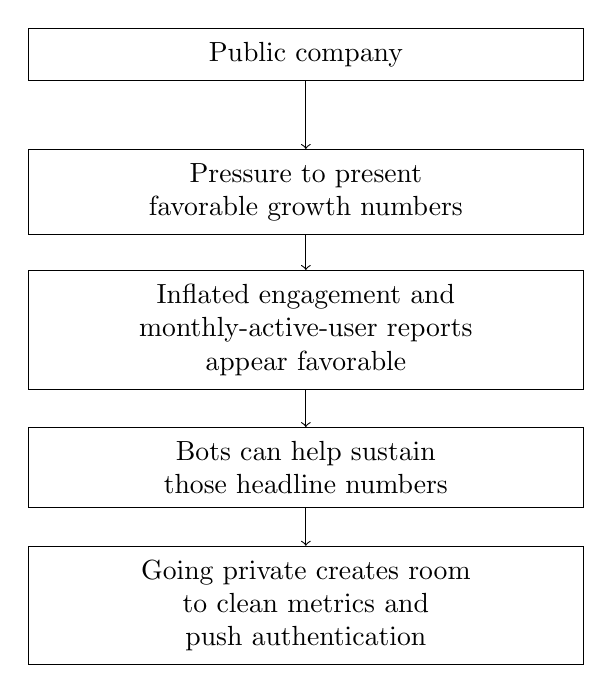
\begin{tikzpicture}
\node[draw, align=center, text width=6.7cm, inner sep=5pt] (n1) at (0,0) {Public company};
\node[draw, align=center, text width=6.7cm, inner sep=5pt] (n2) at (0,-1.75) {Pressure to present\\favorable growth numbers};
\node[draw, align=center, text width=6.7cm, inner sep=5pt] (n3) at (0,-3.5) {Inflated engagement and\\monthly-active-user reports\\appear favorable};
\node[draw, align=center, text width=6.7cm, inner sep=5pt] (n4) at (0,-5.25) {Bots can help sustain\\those headline numbers};
\node[draw, align=center, text width=6.7cm, inner sep=5pt] (n5) at (0,-7.0) {Going private creates room\\to clean metrics and\\push authentication};
\draw[->] (n1) -- (n2);
\draw[->] (n2) -- (n3);
\draw[->] (n3) -- (n4);
\draw[->] (n4) -- (n5);
\end{tikzpicture}
}
\caption{A transcript-derived causal chain behind the lecture's account of bots, metrics, and privatization.}
\end{figure}

The lecture then makes its first return to a deeper theme. Bot removal is not enough. If we really want to clean the numbers, we must decide who is actually on the platform. That leads directly to authentication.

\section{Authentication as the Hidden Infrastructure Layer}

At this point the lecture does something important and worth preserving on the page: it does not treat authentication as a decorative add-on. It treats it as the infrastructure beneath several of the other changes. First it helps remove bots. Later it helps govern speech. Later still it helps route payments to the right creator and preserve trust in the platform's records.

The speaker's analogy is ordinary rather than abstract. A Facebook page still has an identifiable administrator behind it. Something comparable is imagined for Twitter: a person, a business, or at least a traceable content page should stand behind the account. We may sketch that logic as a state diagram.

\begin{figure}[h]
\centering
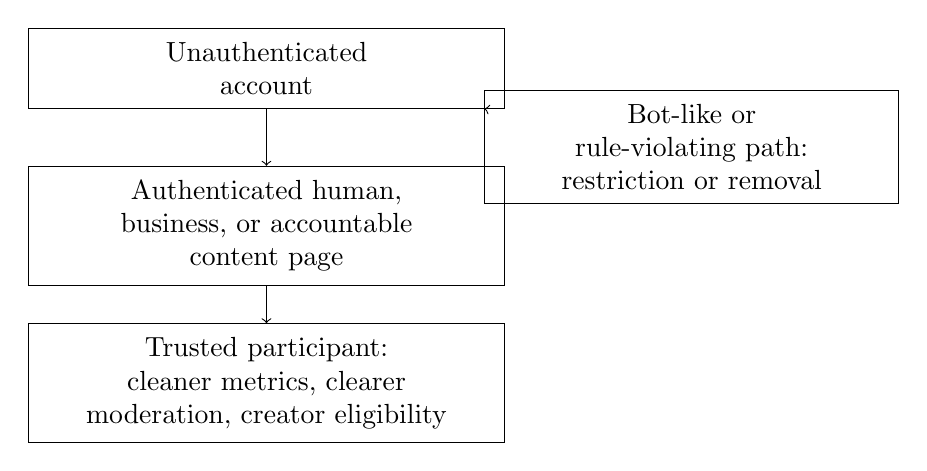
\begin{tikzpicture}
\node[draw, align=center, text width=5.7cm, inner sep=5pt] (u) at (0,0) {Unauthenticated\\account};
\node[draw, align=center, text width=5.7cm, inner sep=5pt] (a) at (0,-2.0) {Authenticated human,\\business, or accountable\\content page};
\node[draw, align=center, text width=5.7cm, inner sep=5pt] (t) at (0,-4.0) {Trusted participant:\\cleaner metrics, clearer\\moderation, creator eligibility};
\node[draw, align=center, text width=4.9cm, inner sep=5pt] (r) at (5.4,-1.0) {Bot-like or\\rule-violating path:\\restriction or removal};
\draw[->] (u) -- (a);
\draw[->] (a) -- (t);
\draw[->] (u) -- (r);
\end{tikzpicture}
\caption{A cautious transcript-derived state diagram for the lecture's authentication layer.}
\end{figure}

To make the governance claim explicit, let \(\mathcal U_A\) be the set of authenticated users and let \(\mathcal R\) be the set of accounts restricted or removed for specified reasons. Then the lecture's underlying rule can be written as
\begin{equation}
S(u) = S_0
\qquad
\forall\, u \in \mathcal U_A \setminus \mathcal R,
\end{equation}
where \(S(u)\) is the service level delivered to user \(u\), and \(S_0\) is the common platform service to be provided when no specific rule has been triggered.

The equation is schematic, but the lecture's point is exact. We are not trying to tailor a separate platform for every political or cultural preference. We are trying to build a platform that knows who is on it and can then apply rules consistently.

That is why authentication sits between the bot discussion and the censorship discussion. First we ask, who is really here? Only then do we ask, how should the platform treat those who are here?

\section{Censorship, Free Speech, and a Rule-Bound Platform}

The lecturer's next move is to free speech, but he arrives there through identity rather than through abstract political principle. Some viewers, he says, worry that pulling back on censorship would let objectionable people speak too freely. He does not deny that concern. Instead, he reframes the target. The goal is not universal approval. The goal is rule-consistent service to authenticated users.

This is where the lecture offers its striking rhetorical balance condition. Musk is said to want the most radical \(10\%\) on each side of the political spectrum to be equally unhappy. If we formalize that claim at all, we should do so very lightly:
\begin{equation}
D_L \approx D_R.
\end{equation}
Here \(D_L\) and \(D_R\) are heuristic dissatisfaction levels at the left and right extremes. This is not empirical measurement. It is a compact expression of the lecture's balancing image: no faction should feel that the platform is uniquely designed for it.

The actual operational claim lies elsewhere. The platform should provide the same service to authenticated users across viewpoints, while still keeping the option to shut accounts down for specific reasons set in advance. In the speaker's language, one does not cater to every opinion, want, or need; one tries to maintain a common service layer and reserve intervention for explicit cases.

That ordering is worth preserving in the final notes. The lecture does not proceed by saying ``free speech is good'' and stopping there. It proceeds more carefully: authentication first, then service symmetry, then limited grounds for removal. In entrepreneurial terms, moderation is being imagined not as mood management but as rule design.

\section{Creator Pay, Web3, and the Economics of Attention}

The third major prediction turns from governance to incentives. If we have cleaned the platform and made participation more legible, the next question is natural: what does the platform reward? The lecture's answer is speculative but structurally clear. Twitter, in the speaker's view, pays creators poorly compared with short-form video platforms. Many accounts still monetize through their own affiliate or marketing strategies rather than through a strong native payout rail.

This is where the lecture introduces the analogy of \emph{play to earn}. In gaming and esports-adjacent economies, one can imagine a system in which playing and performing generate cryptocurrency or other reward. The speaker then asks whether Twitter could move toward a similar \emph{tweet to earn} model. We can summarize that conjecture by writing
\begin{equation}
p_i = f(a_i,g_i),
\qquad
a_i \in \{0,1\},
\end{equation}
where \(p_i\) is the payout to creator \(i\), \(a_i\) is an authentication flag, and \(g_i\) is the creator's engagement. The lecture does not define \(f\), and we should not pretend otherwise. We are only writing down the structure that the speaker has in mind: verification plus engagement produces eligibility for payment.

There is an instructive contrast here. Outside Twitter, short-form platforms are said to pay creators on views and engagement. Inside Twitter, the revenue path is described as more external and more improvised. A creator often brings the monetization mechanism from outside the platform instead of receiving it from the platform itself.

We can see why authentication reappears. Suppose
\[
g_1 = g_2,
\]
so that two accounts draw the same level of engagement. If
\[
a_1 = 1,\qquad a_2 = 0,
\]
then the platform can at least imagine rewarding creator \(1\) while withholding or delaying payout to creator \(2\) until identity is verified. The point is not that Twitter already does this. The point is that once the lecture starts imagining native creator pay, the old theme returns: if we cannot tell who is real, we cannot tell who should be paid.

The speaker then compares Twitter with TikTok, Reels, Shorts, and Snapchat, and even speculates that Musk might someday bring short-form video more directly into Twitter. Those lines remain speculative, and the notes should keep them that way. But the motivational sequence is important: the platform first removes distortion, then identifies users, then asks how genuine productive attention might be rewarded.

\section{Open-Source Algorithm and Operational Transparency}

The fourth prediction is shorter and tighter. The lecture now turns to the platform's algorithm itself. The speaker argues that an open-source algorithm would improve transparency for creators and users by making the logic of ranking and visibility less opaque.

Several practical consequences are then attached to this proposal. Since private ownership is supposed to make redesign easier, the lecturer says that an open-source algorithm could reduce maintenance costs and increase speed, flexibility, and security. We should preserve those claims in the order given, but we should also preserve their status: they are asserted benefits, not proved results.

The placement of this section matters. It arrives after creator pay because the lecture is still asking what sort of infrastructure a rebuilt platform would require. If metrics are to be cleaner, if moderation is to be more rule-bound, and if creators are to be paid more natively, then the system that distributes visibility must eventually be made more legible as well. The algorithmic question is therefore not a technical digression. It is the infrastructure-side continuation of the same entrepreneurial design program.

\section{Edit Button and Historical Integrity}

Before the last move, the lecture briefly pauses and invites the audience to comment on what has been missed. Then it returns with the strongest local puzzle in the entire talk. The final likely change is the addition of an edit button.

The speaker grants immediately why the idea is attractive. Many users seem to want it, and the polling he mentions suggests broad support. But he does not let the topic remain at the level of convenience. He sharpens it at once. On the surface an edit button looks simple; in reality it may threaten the integrity of the original tweet. The design question is no longer, \emph{Should a tweet be editable?} It is, \emph{Can a tweet be editable without losing its historical meaning?}

\subsection{Question \& Answer}

\paragraph{Question.}
How can we allow edits while preserving the authenticity of what was originally stated?

\paragraph{Answer.}
The lecture's answer is to separate the \emph{current visible tweet} from the \emph{history of that tweet}. The visible form may change, but the earlier states must remain inspectable. The speaker uses blockchain language to describe this, but the essential structure is simpler and need not be overstated. What we need is an append-only history.

Let
\begin{equation}
H_n(T)=\bigl(T^{(0)},T^{(1)},\dots,T^{(n)}\bigr)
\end{equation}
be the history of tweet \(T\) through its \(n\)-th version, where \(T^{(0)}\) is the original statement. Then the currently displayed tweet is
\begin{equation}
T_{\mathrm{curr}} = T^{(n)}.
\end{equation}
When an edit occurs, the lecture's logic is not to overwrite the past but to append a new state:
\begin{align}
H_{n+1}(T) &= \bigl(T^{(0)},T^{(1)},\dots,T^{(n)},T^{(n+1)}\bigr), \\
T_{\mathrm{curr}} &\leftarrow T^{(n+1)}.
\end{align}
From that structure the integrity condition follows immediately:
\begin{equation}
T^{(0)} \in H_{n+1}(T)
\qquad
\text{even though}
\qquad
T_{\mathrm{curr}} \neq T^{(0)}.
\end{equation}

This is the cleanest mathematical moment in the chapter, not because it uses advanced mathematics, but because it isolates the design principle exactly. Editing and authenticity are compatible only if the platform preserves lineage. The present may be revised, but the past must remain reachable.

\begin{figure}[h]
\centering
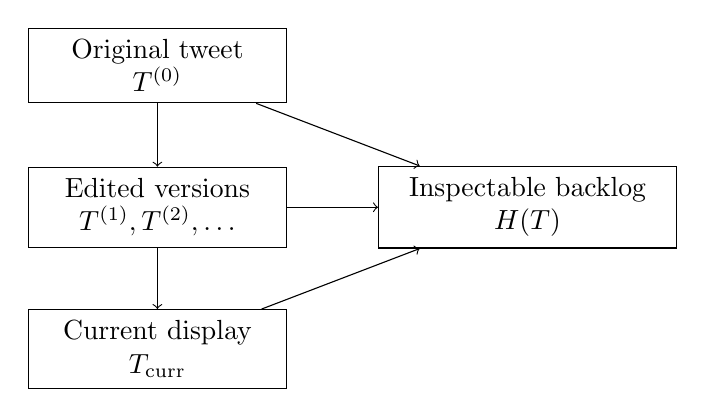
\begin{tikzpicture}
\node[draw, align=center, text width=3.0cm, inner sep=4pt] (o) at (0,0) {Original tweet\\\(T^{(0)}\)};
\node[draw, align=center, text width=3.0cm, inner sep=4pt] (e) at (0,-1.8) {Edited versions\\\(T^{(1)},T^{(2)},\dots\)};
\node[draw, align=center, text width=3.0cm, inner sep=4pt] (c) at (0,-3.6) {Current display\\\(T_{\mathrm{curr}}\)};
\node[draw, align=center, text width=3.5cm, inner sep=4pt] (h) at (4.7,-1.8) {Inspectable backlog\\\(H(T)\)};
\draw[->] (o) -- (e);
\draw[->] (e) -- (c);
\draw[->] (o) -- (h);
\draw[->] (e) -- (h);
\draw[->] (c) -- (h);
\end{tikzpicture}
\caption{A transcript-derived model of editable tweets with preserved version history.}
\end{figure}

We should also notice how the lecture closes a circle here. The platform began as a question of trust: are the accounts real, are the metrics real, are the moderation rules real, are the payouts going to the right place? The edit button returns us to exactly the same theme, now in textual form. Can the platform change without letting history disappear?

The lecturer's answer is modest and precise. We need not insist on blockchain in the strong technical sense. What matters is the append-only logic. The current tweet can evolve, but its ancestry must remain visible. That is the condition under which convenience does not erase accountability.

\section{Summary}

The lecture starts with public controversy and ends with historical integrity, but the movement between those points is more coherent than it first appears. First, bot activity is treated as a distortion of engagement and monthly-active-user counts, so the platform's visible success becomes entangled with contaminated metrics. Second, authentication emerges as the hidden infrastructure beneath everything else: it supports cleaner accounting, more legible moderation, more credible creator pay, and more trustworthy records. Third, reduced censorship is framed not as universal approval, but as equal service under rules. Fourth, creator economics is reimagined through a speculative tweet-to-earn logic that borrows its metaphor from gaming and its competitive pressure from short-form platforms. Fifth, an open-source algorithm is offered as a route to transparency and operational flexibility. Finally, the edit button becomes the lecture's sharpest design problem, resolved by the idea of an inspectable backlog of prior versions.

Read as entrepreneurship notes, the chapter is therefore not chiefly about Musk as a personality. It is about ownership as a chance to redesign a system. The five predictions are really five questions about incentives and trust: what is being counted, who is being counted, how rules are applied, how attention is rewarded, how visibility is governed, and how a platform preserves memory while permitting change.
